\documentclass[11pt,a4paper]{article}

\usepackage[margin=2.2cm]{geometry}
\usepackage[T1]{fontenc}
\usepackage[utf8]{inputenc}
\usepackage{lmodern}
\usepackage{amsmath,amssymb,mathtools}
\usepackage{booktabs}
\usepackage{array}
\usepackage{enumitem}
\usepackage{hyperref}
\usepackage{xcolor}
\usepackage{tikz}
\usetikzlibrary{arrows.meta,positioning,fit,calc}

\hypersetup{
  colorlinks=true,
  linkcolor=blue!50!black,
  urlcolor=blue!50!black
}

\title{How \texttt{C\_OtherCombustion} Works\\
\large Step-by-step algorithm, formulas, and interpretation of the final pollutant weight rasters}
\author{}
\date{\today}

\newcommand{\R}{\mathbb{R}}
\newcommand{\eps}{\varepsilon}

\begin{document}
\maketitle

\section{Purpose}

This note explains, step by step, what the code in
\texttt{PROXY/sectors/C\_OtherCombustion/} does, which formulas it implements,
and how it produces the final per-pollutant weight rasters written by the
pipeline.

The sector allocates CAMS GNFR C emissions from source cells onto the reference
grid by combining:

\begin{itemize}[leftmargin=1.4em]
  \item \textbf{spatial proxy fields} from Hotmaps, CORINE, and optional rural bias,
  \item \textbf{activity and appliance information} from GAINS,
  \item \textbf{emission factors} from EMEP,
  \item \textbf{household/commercial end-use weights} from Eurostat.
\end{itemize}

At the highest level, the code builds two ingredients:

\begin{enumerate}[leftmargin=1.4em]
  \item a spatial proxy tensor $X$ on the reference grid,
  \item a pollutant-by-class matrix $M$,
\end{enumerate}

and then, for each CAMS source cell, computes
\[
U = X_w M^\top,
\]
normalizes each pollutant column of $U$ to shares, multiplies by the CAMS
emission of that pollutant, and accumulates the result on the reference grid.

\section{Files and responsibilities}

\begin{center}
\begin{tabular}{p{0.28\linewidth}p{0.62\linewidth}}
\toprule
\textbf{File} & \textbf{Role} \\
\midrule
\texttt{builder.py} & Merge config, build the reference window, call the pipeline. \\
\texttt{pipeline.py} & Orchestrate the whole run, loop over CAMS cells, write outputs. \\
\texttt{x\_builder/hotmaps\_base.py} & Build residential and commercial base rasters from Hotmaps heat and GFA. \\
\texttt{x\_builder/corine\_morphology.py} & Convert CORINE classes into morphology multipliers. \\
\texttt{x\_builder/rural\_bias.py} & Build optional rural enhancement factor from population or GHSL. \\
\texttt{x\_builder/stack.py} & Assemble the final $X$ tensor with 7 model-class bands. \\
\texttt{m\_builder/enduse\_factors.py} & Compute Eurostat-based end-use weights and GAINS appliance splits. \\
\texttt{m\_builder/assemble.py} & Build the matrix $M[p,k]$. \\
\texttt{allocator.py} & Normalize $U$ per pollutant and scatter-add emissions and weights. \\
\texttt{constants.py} & Define the 7 model classes and their fixed order. \\
\bottomrule
\end{tabular}
\end{center}

\section{Notation}

\subsection{Model classes}

The code uses exactly 7 model classes in the fixed order
\[
k \in \{
\texttt{R\_FIREPLACE},
\texttt{R\_HEATING\_STOVE},
\texttt{R\_COOKING\_STOVE},
\texttt{R\_BOILER\_MAN},
\texttt{R\_BOILER\_AUT},
\texttt{C\_BOILER\_MAN},
\texttt{C\_BOILER\_AUT}
\}.
\]

We will denote the total number of classes by $K=7$.

\subsection{Grid and tensor shapes}

\begin{itemize}[leftmargin=1.4em]
  \item The reference raster has height $H$ and width $W$.
  \item The number of requested output pollutants is $P$.
  \item The proxy stack is
  \[
  X \in \R^{H \times W \times K}.
  \]
  \item For one CAMS cell, after intersecting with the reference grid window, the
  overlapping pixels are flattened into
  \[
  X_w \in \R^{n_{\text{pix}} \times K}.
  \]
  \item For one country, the pollutant-by-class matrix is
  \[
  M \in \R^{P \times K}.
  \]
  \item The per-pixel, per-pollutant pre-normalization scores are
  \[
  U = X_w M^\top \in \R^{n_{\text{pix}} \times P}.
  \]
\end{itemize}

\subsection{Two different outputs to keep distinct}

The code maintains two different accumulators:

\begin{enumerate}[leftmargin=1.4em]
  \item \textbf{Allocated emissions}
  \[
  A \in \R^{P \times H \times W},
  \]
  stored in \texttt{acc}, containing pollutant mass in kg/yr.

  \item \textbf{Weight rasters}
  \[
  W \in \R^{P \times H \times W},
  \]
  stored in \texttt{weights\_acc}, containing the \emph{sum of local per-cell
  shares} added by all contributing CAMS cells.
\end{enumerate}

This second point is important: the final written weight raster is \emph{not}
globally normalized to sum to 1 over the whole country. It is the sum of
within-cell normalized shares over all processed CAMS cells.

\section{End-to-end pipeline}

\begin{figure}[ht]
\centering
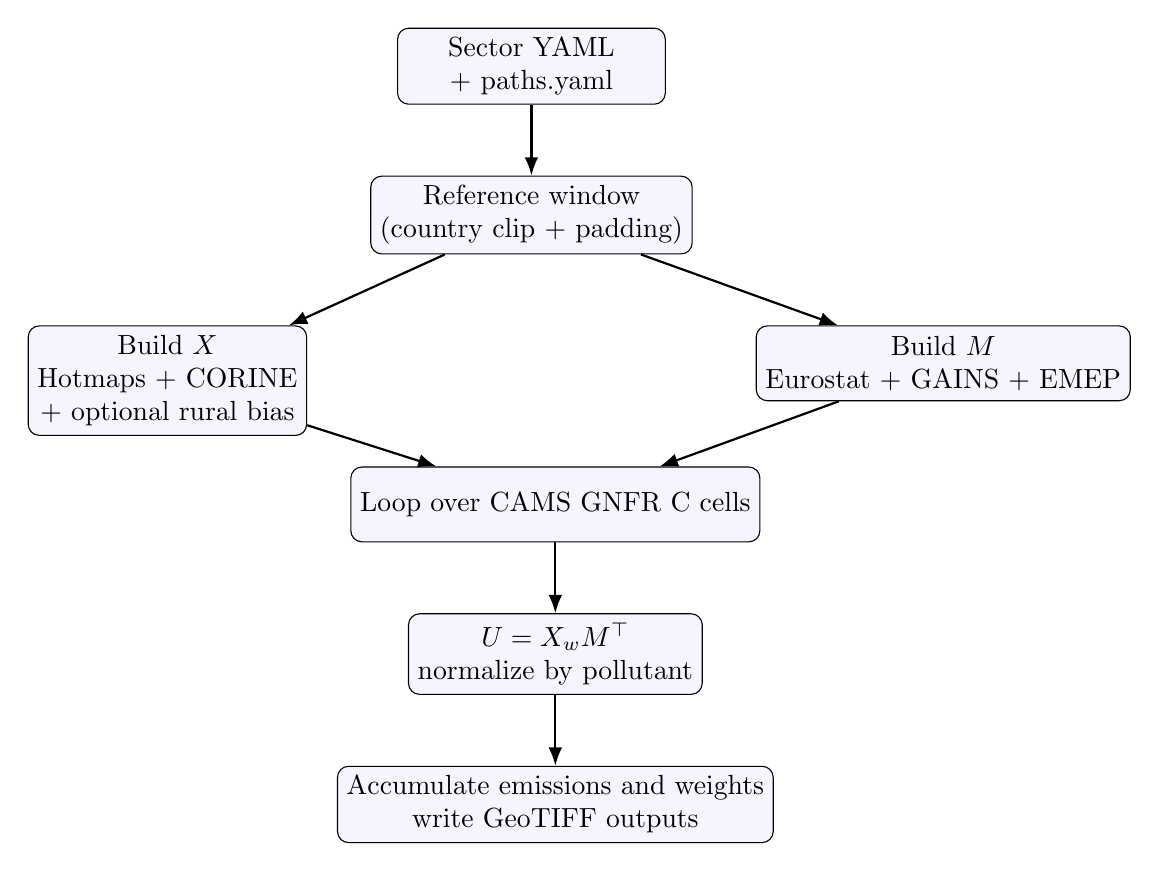
\begin{tikzpicture}[
  node distance=0.9cm and 0.8cm,
  box/.style={draw, rounded corners, align=center, minimum width=3.4cm, minimum height=0.95cm, fill=blue!4},
  arr/.style={-Latex, thick}
]
\node[box] (cfg) {Sector YAML\\ + paths.yaml};
\node[box, below=of cfg] (ref) {Reference window\\ (country clip + padding)};
\node[box, below left=of ref] (x) {Build $X$\\ Hotmaps + CORINE\\ + optional rural bias};
\node[box, below right=of ref] (m) {Build $M$\\ Eurostat + GAINS + EMEP};
\node[box, below=1.2cm of $(x)!0.5!(m)$] (cams) {Loop over CAMS GNFR C cells};
\node[box, below=of cams] (u) {$U = X_w M^\top$\\ normalize by pollutant};
\node[box, below=of u] (out) {Accumulate emissions and weights\\ write GeoTIFF outputs};

\draw[arr] (cfg) -- (ref);
\draw[arr] (ref) -- (x);
\draw[arr] (ref) -- (m);
\draw[arr] (x) -- (cams);
\draw[arr] (m) -- (cams);
\draw[arr] (cams) -- (u);
\draw[arr] (u) -- (out);
\end{tikzpicture}
\caption{High-level structure of the implementation.}
\end{figure}

\section{Step 1: build the reference window}

In \texttt{builder.py}, the code first constructs a reference raster profile
using the selected NUTS country, the CORINE raster, and a padding distance.
This fixes:

\begin{itemize}[leftmargin=1.4em]
  \item the output CRS,
  \item the affine transform,
  \item the raster size $(H,W)$,
  \item the WGS84 bounding box of the domain.
\end{itemize}

Everything else is warped or sliced onto this reference geometry.

\section{Step 2: build the spatial proxy tensor $X$}

\subsection{2.1 Hotmaps base rasters}

The code warps four rasters to the reference grid:

\begin{itemize}[leftmargin=1.4em]
  \item residential heat density $H_{\mathrm{res}}$,
  \item non-residential heat density $H_{\mathrm{com}}$,
  \item residential gross floor area $G_{\mathrm{res}}$,
  \item non-residential gross floor area $G_{\mathrm{com}}$.
\end{itemize}

From those, it computes a residential base field $R_{\mathrm{base}}$ and a
commercial base field $C_{\mathrm{base}}$ using one of two formulas.

\paragraph{Multiplicative mode}
If \texttt{use\_additive\_instead = false}, the code applies
\[
R_{\mathrm{base}}(q) =
\bigl(H_{\mathrm{res}}(q)+\eps\bigr)^{a_h}
\bigl(G_{\mathrm{res}}(q)+\eps\bigr)^{a_g},
\]
\[
C_{\mathrm{base}}(q) =
\bigl(H_{\mathrm{com}}(q)+\eps\bigr)^{a_h}
\bigl(G_{\mathrm{com}}(q)+\eps\bigr)^{a_g},
\]
where $a_h=\texttt{heat\_exp}$, $a_g=\texttt{gfa\_exp}$, and
$\eps=\texttt{epsilon}$.

\paragraph{Additive mode}
If \texttt{use\_additive\_instead = true}, the code instead uses
\[
R_{\mathrm{base}}(q) = w_h H_{\mathrm{res}}(q) + w_g G_{\mathrm{res}}(q),
\]
\[
C_{\mathrm{base}}(q) = w_h H_{\mathrm{com}}(q) + w_g G_{\mathrm{com}}(q),
\]
with $w_h=\texttt{additive\_heat\_weight}$ and
$w_g=\texttt{additive\_gfa\_weight}$.

Negative values are clipped to zero before these formulas are applied.

\subsection{2.2 CORINE morphology}

The CORINE raster is warped to the same reference grid, decoded to level-3 land
cover classes, and turned into the indicator masks
\[
u_{111}, \quad u_{112}, \quad u_{121},
\]
where each mask is 1 on the corresponding CORINE class and 0 elsewhere.

The code then defines an ``other'' mask:
\[
u_{\mathrm{other}} = \mathrm{clip}(1 - u_{111} - u_{112} - u_{121}, 0, 1).
\]

From the YAML morphology coefficients it constructs:

\paragraph{Residential morphology}
\[
m_r =
w^{(r)}_{111} u_{111}
 w^{(r)}_{112} u_{112}
 w^{(r)}_{\mathrm{other}} u_{\mathrm{other}}.
\]

\paragraph{Commercial morphology}
\[
m_c =
w^{(c)}_{111} u_{111}
 w^{(c)}_{121} u_{121}
 w^{(c)}_{\mathrm{other}} u_{\mathrm{other}}.
\]

So CORINE does not directly allocate pollutant mass; it modulates the spatial
proxy intensity used later in $X$.

\subsection{2.3 Optional rural bias}

If \texttt{rural\_bias.enabled = true}, the code warps either a population raster
or a GHSL settlement raster, then computes:
\[
z(q) = \log\bigl(1 + d(q)\bigr),
\]
followed by min-max normalization over valid positive cells:
\[
s_0(q) = \frac{z(q)-z_{\min}}{z_{\max}-z_{\min}},
\]
with the special-case behavior implemented in the code if $z_{\max} \le z_{\min}$.

Then a $5 \times 5$ mean filter is applied:
\[
s(q) = \mathrm{smooth}_{5 \times 5}\bigl(s_0(q)\bigr).
\]

Finally the rural-bias multiplier is
\[
r_b(q) = \mathrm{clip}\bigl(1-s(q),\ r_{\min},\ 1\bigr),
\]
where $r_{\min}=\texttt{rural\_min}$.

In the current implementation this factor is only applied to the configured
residential fireplace and heating-stove bands.

\subsection{2.4 Final 7-band tensor $X$}

The 7 bands of $X$ are filled exactly as follows:

\[
X(:,:,0) = R_{\mathrm{base}} \cdot m_r \cdot r_b^{(0)},
\]
\[
X(:,:,1) = R_{\mathrm{base}} \cdot m_r \cdot r_b^{(1)},
\]
\[
X(:,:,2) = R_{\mathrm{base}},
\qquad
X(:,:,3) = R_{\mathrm{base}},
\qquad
X(:,:,4) = R_{\mathrm{base}},
\]
\[
X(:,:,5) = C_{\mathrm{base}} \cdot m_c,
\qquad
X(:,:,6) = C_{\mathrm{base}} \cdot m_c.
\]

Here $r_b^{(0)}$ and $r_b^{(1)}$ are either the rural-bias raster or 1, depending
on whether the corresponding class index is listed in the rural-bias class list.

Therefore:

\begin{itemize}[leftmargin=1.4em]
  \item morphology affects only fireplace/heating-stove residential bands and both commercial boiler bands,
  \item rural bias affects only the selected residential bands,
  \item cooking and residential boiler bands currently use the residential base
  field without a separate morphology factor.
\end{itemize}

\section{Step 3: build Eurostat end-use and GAINS appliance factors}

\subsection{3.1 Bucket mapping}

Each model class $k$ is assigned to an end-use bucket $b(k)$:

\begin{itemize}[leftmargin=1.4em]
  \item every commercial class maps to the bucket \texttt{commercial},
  \item residential classes map according to \texttt{eurostat\_end\_use.json},
  \item a class may also map to a default residential bucket or to a composite
  bucket such as \texttt{space\_heating|water\_heating}.
\end{itemize}

\paragraph{What is an end-use bucket?}
An \emph{end-use bucket} is simply a coarse label for the \textbf{purpose} for which
energy is used, not the appliance itself and not the fuel. In the Eurostat dataset
\texttt{nrg\_d\_hhq}, the residential energy of households is split into broad uses such as:

\begin{itemize}[leftmargin=1.4em]
  \item \texttt{space\_heating},
  \item \texttt{water\_heating},
  \item \texttt{cooking},
  \item \texttt{space\_cooling},
  \item \texttt{lighting\_appliances},
  \item \texttt{other\_end\_use}.
\end{itemize}

So an end-use bucket answers the question:

\begin{quote}
``What is the energy used \textbf{for}?'' 
\end{quote}

By contrast, a GAINS row is closer to:

\begin{quote}
``Which \textbf{technology / appliance / fuel combination} is responsible?''
\end{quote}

For example:

\begin{itemize}[leftmargin=1.4em]
  \item Eurostat says: a certain share of household energy goes to \texttt{cooking}.
  \item GAINS says: some share of activity is in \emph{Cooking stoves} using \emph{Gas oil}.
\end{itemize}

Those are not the same type of object, which is why the code needs an intermediate layer.

\paragraph{The crucial idea}
The code does \textbf{not} directly map Eurostat categories to raw GAINS rows.
Instead, it uses the \textbf{7 model classes} as the bridge:

\[
\text{Eurostat end-use bucket}
\longrightarrow
\text{model class}
\longleftarrow
\text{GAINS row}.
\]

That is the key to understanding Step 3.

\subsection{3.1.1 The two mappings used by the code}

There are really two separate mappings:

\paragraph{Mapping A: GAINS row $\rightarrow$ model class}
This is defined in \texttt{GAINS\_mapping.json}. A rule looks at the GAINS
\texttt{fuel} string and the GAINS \texttt{appliance} string, and assigns the row
to one of the 7 classes. For example:

\begin{itemize}[leftmargin=1.4em]
  \item ``Cooking stoves'' + ``(households)'' + fuel match $\rightarrow$ \texttt{R\_COOKING\_STOVE},
  \item ``Fireplaces'' + ``(households)'' + fuel match $\rightarrow$ \texttt{R\_FIREPLACE},
  \item ``Single house boilers'' + ``automatic'' $\rightarrow$ \texttt{R\_BOILER\_AUT},
  \item ``Medium boilers'' + ``(commercial)'' + ``manual'' $\rightarrow$ \texttt{C\_BOILER\_MAN}.
\end{itemize}

\paragraph{Mapping B: model class $\rightarrow$ Eurostat end-use bucket}
This is defined in \texttt{eurostat\_end\_use.json} through \texttt{class\_to\_metric}.
For the current project configuration, it is:

\begin{center}
\begin{tabular}{lll}
\toprule
\textbf{Model class} & \textbf{Eurostat bucket} & \textbf{Interpretation} \\
\midrule
\texttt{R\_FIREPLACE} & \texttt{space\_heating} & Residential fireplace used for heating \\
\texttt{R\_HEATING\_STOVE} & \texttt{space\_heating} & Residential heating stove \\
\texttt{R\_COOKING\_STOVE} & \texttt{cooking} & Residential cooking \\
\texttt{R\_BOILER\_MAN} & \texttt{space\_heating|water\_heating} & Shared across two household uses \\
\texttt{R\_BOILER\_AUT} & \texttt{space\_heating|water\_heating} & Shared across two household uses \\
\texttt{C\_BOILER\_MAN} & \texttt{commercial} & Commercial total \\
\texttt{C\_BOILER\_AUT} & \texttt{commercial} & Commercial total \\
\bottomrule
\end{tabular}
\end{center}

\paragraph{What this means conceptually}
Eurostat tells the code how much \emph{total residential energy demand} belongs to
each broad use. GAINS tells the code how that activity is distributed among more
specific appliance classes. The model class is the place where those two views meet.

\subsection{3.1.2 Why this indirection is needed}

Suppose Eurostat says that in a given country:

\begin{itemize}[leftmargin=1.4em]
  \item 60\% of household energy is for space heating,
  \item 10\% is for water heating,
  \item 5\% is for cooking,
  \item the rest is for other uses.
\end{itemize}

Eurostat does \emph{not} tell us how the space-heating share should be split between:

\begin{itemize}[leftmargin=1.4em]
  \item fireplaces,
  \item heating stoves,
  \item manual boilers,
  \item automatic boilers.
\end{itemize}

That finer split is taken from GAINS. So the logic is:

\begin{enumerate}[leftmargin=1.4em]
  \item use Eurostat to say how much weight belongs to each \emph{broad end use},
  \item use GAINS to divide that broad end-use total among the model classes that
  live inside that bucket.
\end{enumerate}

In short:
\[
\text{Eurostat gives the size of the pie,}
\qquad
\text{GAINS cuts the pie among classes.}
\]

\subsection{3.2 Commercial share from \texttt{nrg\_bal\_s}}

The code fetches Eurostat total final energy for:
\[
\mathrm{CP} = \texttt{FC\_OTH\_CP\_E},
\qquad
\mathrm{HH} = \texttt{FC\_OTH\_HH\_E}.
\]

It defines the commercial fraction
\[
\alpha = \frac{\mathrm{CP}}{\mathrm{CP} + \mathrm{HH}}.
\]

If this value is unavailable, the code falls back to
\[
\alpha = 0.
\]

\subsection{3.3 Residential end-use decomposition from \texttt{nrg\_d\_hhq}}

Let the six Eurostat residential household metrics be denoted by
\[
m \in \{
\texttt{space\_heating},
\texttt{water\_heating},
\texttt{cooking},
\texttt{space\_cooling},
\texttt{lighting\_appliances},
\texttt{other\_end\_use}
\}.
\]

The code fetches TJ values $T_m$ for these six metrics and defines the total
residential fraction
\[
f_{\mathrm{res}} = \max(0, \min(1, 1-\alpha)).
\]

If the total household TJ is positive, then
\[
f_{\mathrm{enduse}}(m) = f_{\mathrm{res}} \frac{T_m}{\sum_{m'} T_{m'}}.
\]

If no positive residential TJ values are available, the code falls back to a flat
split based on the configured default residential multiplier:
\[
f_{\mathrm{enduse}}(m) =
\frac{\texttt{default\_residential\_if\_missing} \cdot f_{\mathrm{res}}}{6}.
\]

For the commercial bucket:
\[
f_{\mathrm{enduse}}(\texttt{commercial}) = \alpha.
\]

Composite residential buckets such as
\texttt{space\_heating|water\_heating} are implemented as the arithmetic mean of
their component buckets.

\subsection{3.4 Appliance fractions from GAINS}

The code also uses the focus country's GAINS table to aggregate activity shares by
model class:
\[
a_k = \sum_{r \in \mathcal{R}_k} s_r,
\]
where each row $r$ mapped to class $k$ contributes its GAINS share $s_r$.

Then, within each end-use bucket $b$, the code defines the normalized appliance split:
\[
f_{\mathrm{appliance}}(k) =
\frac{a_k}{\sum_{k' : b(k') = b(k)} a_{k'}}.
\]

If the denominator is zero, it falls back to
\[
f_{\mathrm{appliance}}(k) = 1.
\]

\paragraph{This is the exact link between Eurostat and GAINS}
This is the part that is easiest to miss when reading the code.

The code first computes a Eurostat weight at the \textbf{bucket level}:
\[
f_{\mathrm{enduse}}(b).
\]

Then it computes a GAINS-based split \emph{within that same bucket}:
\[
f_{\mathrm{appliance}}(k)
=
\frac{\text{GAINS activity of class }k}
{\text{total GAINS activity of all classes in the same bucket}}.
\]

Then the class-level multiplier becomes
\[
\rho_k = f_{\mathrm{enduse}}(b(k)) \cdot f_{\mathrm{appliance}}(k).
\]

So the Eurostat total is first assigned to the bucket, and only then divided across
the classes that belong to that bucket.

\subsection{3.4.1 Worked example: space heating}

Assume the current mapping:

\begin{itemize}[leftmargin=1.4em]
  \item \texttt{R\_FIREPLACE} $\rightarrow$ \texttt{space\_heating},
  \item \texttt{R\_HEATING\_STOVE} $\rightarrow$ \texttt{space\_heating},
  \item \texttt{R\_BOILER\_MAN}, \texttt{R\_BOILER\_AUT} $\rightarrow$ \texttt{space\_heating|water\_heating}.
\end{itemize}

Suppose Eurostat gives:
\[
f_{\mathrm{enduse}}(\texttt{space\_heating}) = 0.50,
\qquad
f_{\mathrm{enduse}}(\texttt{water\_heating}) = 0.10.
\]

Then for boiler classes, the code creates the composite bucket:
\[
f_{\mathrm{enduse}}(\texttt{space\_heating|water\_heating})
= \frac{0.50 + 0.10}{2} = 0.30.
\]

Now suppose the GAINS activity sums for the relevant classes are:
\[
a_{\texttt{R\_FIREPLACE}} = 2,
\qquad
a_{\texttt{R\_HEATING\_STOVE}} = 18.
\]

Because both of these classes belong to the same bucket \texttt{space\_heating},
the code normalizes them within that bucket:
\[
f_{\mathrm{appliance}}(\texttt{R\_FIREPLACE}) = \frac{2}{2+18} = 0.1,
\]
\[
f_{\mathrm{appliance}}(\texttt{R\_HEATING\_STOVE}) = \frac{18}{2+18} = 0.9.
\]

Therefore their final row multipliers are:
\[
\rho_{\texttt{R\_FIREPLACE}} = 0.50 \times 0.10 = 0.05,
\]
\[
\rho_{\texttt{R\_HEATING\_STOVE}} = 0.50 \times 0.90 = 0.45.
\]

Interpretation:

\begin{itemize}[leftmargin=1.4em]
  \item Eurostat says: space heating is important overall.
  \item GAINS says: within space-heating technologies, heating stoves are much more important than fireplaces.
  \item The code combines both statements by assigning most of the
  \texttt{space\_heating} bucket to \texttt{R\_HEATING\_STOVE}.
\end{itemize}

\subsection{3.4.2 Worked example: cooking}

If \texttt{R\_COOKING\_STOVE} is the only class mapped to \texttt{cooking}, then:
\[
f_{\mathrm{appliance}}(\texttt{R\_COOKING\_STOVE}) = 1.
\]

So in that case:
\[
\rho_{\texttt{R\_COOKING\_STOVE}}
= f_{\mathrm{enduse}}(\texttt{cooking}).
\]

This is why some classes inherit a bucket almost directly, while others share it.

\subsection{3.4.3 Worked example: commercial}

Both commercial classes map to the same bucket:
\[
\texttt{C\_BOILER\_MAN},\ \texttt{C\_BOILER\_AUT}
\rightarrow \texttt{commercial}.
\]

If Eurostat gives commercial share $\alpha$, then:
\[
f_{\mathrm{enduse}}(\texttt{commercial}) = \alpha.
\]

Suppose GAINS says:
\[
a_{\texttt{C\_BOILER\_MAN}} = 0.2,
\qquad
a_{\texttt{C\_BOILER\_AUT}} = 0.8.
\]

Then:
\[
f_{\mathrm{appliance}}(\texttt{C\_BOILER\_MAN}) = 0.2,
\qquad
f_{\mathrm{appliance}}(\texttt{C\_BOILER\_AUT}) = 0.8,
\]
and therefore
\[
\rho_{\texttt{C\_BOILER\_MAN}} = 0.2\alpha,
\qquad
\rho_{\texttt{C\_BOILER\_AUT}} = 0.8\alpha.
\]

\subsection{3.4.4 What is \emph{not} happening}

To avoid a common misunderstanding, the code is \textbf{not} doing any of the following:

\begin{itemize}[leftmargin=1.4em]
  \item it is not matching each Eurostat metric to one specific GAINS CSV row,
  \item it is not replacing GAINS activity shares with Eurostat shares,
  \item it is not using Eurostat to distinguish fuels,
  \item it is not reading appliance-level end-use fractions from Eurostat.
\end{itemize}

Instead, the logic is:

\begin{enumerate}[leftmargin=1.4em]
  \item GAINS row $\rightarrow$ model class,
  \item model class $\rightarrow$ Eurostat bucket,
  \item Eurostat sets the total weight of each bucket,
  \item GAINS splits that bucket across classes,
  \item EMEP converts class activity into pollutant-specific factors.
\end{enumerate}

\subsection{3.5 Final row multiplier}

For each class $k$, the multiplier used later in $M$ is
\[
\rho_k = f_{\mathrm{enduse}}\bigl(b(k)\bigr)\, f_{\mathrm{appliance}}(k).
\]

If Eurostat is disabled or unavailable at the country-label level, the code falls
back to a legacy-uniform mode:
\[
\rho_k = 1 \qquad \text{for all } k.
\]

\paragraph{Important implementation detail}
In the current code, \texttt{compute\_end\_use\_factors()} is called once using the
focus country from the build configuration. The resulting factors $\rho_k$ are then
reused when building $M$ for all countries present in the selected CAMS cells.
Country-to-country variation in $M$ therefore comes from GAINS rows and EMEP factors,
while the Eurostat-driven end-use multipliers are computed once per run.

\section{Step 4: build the pollutant-by-class matrix $M$}

For a given country and a given pollutant $p$, the code loops over GAINS rows
$(\text{fuel}, \text{appliance}, s_r)$, maps each row to a model class $k$, and adds:
\[
M_{p,k}
\mathrel{+}= s_r \, \rho_k \, \mathrm{EF}_p(\text{fuel}, \text{appliance}).
\]

Equivalently,
\[
M_{p,k} =
\sum_{r \in \mathcal{R}_k}
s_r \, \rho_k \, \mathrm{EF}_{p,r}.
\]

Here:

\begin{itemize}[leftmargin=1.4em]
  \item $s_r$ is the normalized GAINS share for row $r$,
  \item $\rho_k$ is the Eurostat-times-appliance multiplier from the previous section,
  \item $\mathrm{EF}_{p,r}$ is the EMEP emission factor in kg/TJ selected for
  pollutant $p$, fuel, and appliance.
\end{itemize}

\subsection{4.1 Meaning of $s_r$}

$s_r$ comes from one row of the GAINS country CSV after reading the selected year
column and converting the percentage to a fraction between 0 and 1.

For example, in the Austria GAINS file one row is:

\begin{quote}
\texttt{Brown coal/lignite grade 1},\\
\texttt{Single house boilers (<50 kW) - manual (households)},\\
\texttt{2020 = 66.67}
\end{quote}

The code converts this to
\[
s_r = \frac{66.67}{100} = 0.6667.
\]

So $s_r$ means:

\begin{quote}
For this specific fuel, what share of the GAINS activity is assigned to this
specific appliance row?
\end{quote}

It is therefore a \textbf{row-level activity share}. It is not yet:

\begin{itemize}[leftmargin=1.4em]
  \item an end-use bucket share from Eurostat,
  \item an emission factor,
  \item a spatial allocation weight,
  \item a final class total.
\end{itemize}

\subsection{4.2 Example of one row entering $M$}

Take again the Austria row:

\begin{itemize}[leftmargin=1.4em]
  \item fuel = \texttt{Brown coal/lignite grade 1},
  \item appliance = \texttt{Single house boilers (<50 kW) - manual (households)},
  \item GAINS value in the chosen year = \texttt{66.67},
  \item hence $s_r = 0.6667$.
\end{itemize}

Using \texttt{GAINS\_mapping.json}, this row maps to
\[
k = \texttt{R\_BOILER\_MAN}.
\]

Suppose Step 3 has already provided
\[
\rho_{\texttt{R\_BOILER\_MAN}} = 0.30.
\]

Now pick one pollutant, say NO$_x$, and suppose the EMEP lookup for this fuel and
appliance gives
\[
\mathrm{EF}_{\text{NO}_x,r} = 120 \ \mathrm{kg/TJ}.
\]

Then this single GAINS row contributes
\[
\Delta M_{\text{NO}_x,\texttt{R\_BOILER\_MAN}}
= s_r \, \rho_k \, \mathrm{EF}_{\text{NO}_x,r}
= 0.6667 \times 0.30 \times 120
= 24.0.
\]

So this row adds 24.0 to the matrix entry for pollutant NO$_x$ and class
\texttt{R\_BOILER\_MAN}.

\subsection{4.3 Why several rows can contribute to the same class}

Many different GAINS rows can map to the same class $k$. For example, manual
residential boilers can appear with different fuels. Each such row has:

\begin{itemize}[leftmargin=1.4em]
  \item its own share $s_r$,
  \item the same class-level multiplier $\rho_k$ once the class is fixed,
  \item its own pollutant EF if the fuel/appliance combination changes.
\end{itemize}

Therefore the final matrix entry is a sum of row contributions:
\[
M_{p,\texttt{R\_BOILER\_MAN}}
= \sum_{r \in \mathcal{R}_{\texttt{R\_BOILER\_MAN}}}
s_r \, \rho_{\texttt{R\_BOILER\_MAN}} \, \mathrm{EF}_{p,r}.
\]

This is exactly why fuel type matters in $M$: different rows in the same class can
have different EMEP emission factors and therefore contribute different amounts.

If a row cannot be mapped to a class, or if its share is non-positive, it is skipped.
If the GAINS file for a country is missing, the matrix for that country is the zero matrix.

\section{Step 5: select CAMS cells}

After opening the CAMS NetCDF, the pipeline builds a mask that keeps only source cells
that satisfy all configured criteria:

\begin{itemize}[leftmargin=1.4em]
  \item inside the domain/country mask,
  \item matching GNFR category C,
  \item matching the requested source types (\texttt{area}, \texttt{point}, or both).
\end{itemize}

Each selected source cell $m$ has:

\begin{itemize}[leftmargin=1.4em]
  \item a longitude/latitude bounding box,
  \item a country ID,
  \item pollutant emissions $E_p^{(m)}$ read from CAMS variables.
\end{itemize}

\section{Step 6: for each CAMS cell, compute $U = X_w M^\top$}

For one selected cell $m$, the code:

\begin{enumerate}[leftmargin=1.4em]
  \item converts the CAMS lon/lat box to the output CRS,
  \item intersects it with the reference raster window,
  \item extracts the overlapping part of $X$,
  \item reshapes that window to
  \[
  X_w^{(m)} \in \R^{n_m \times K},
  \]
  where $n_m$ is the number of overlapping reference pixels,
  \item looks up the appropriate country matrix
  \[
  M^{(m)} \in \R^{P \times K},
  \]
  \item computes
  \[
  U^{(m)} = X_w^{(m)} \bigl(M^{(m)}\bigr)^\top \in \R^{n_m \times P}.
  \]
\end{enumerate}

Expanded by components:
\[
U^{(m)}_{j,p}
= \sum_{k=1}^K X^{(m)}_{w,j,k} \, M^{(m)}_{p,k},
\]
where $j$ indexes the overlapping pixels of CAMS cell $m$.

Interpretation:

\begin{itemize}[leftmargin=1.4em]
  \item $X$ says \emph{where} different combustion classes are spatially plausible,
  \item $M$ says \emph{how strongly} each class contributes to each pollutant,
  \item $U$ combines those two ingredients into per-pixel pollutant scores.
\end{itemize}

\section{Step 7: normalize $U$ to local shares}

For each pollutant $p$ and cell $m$, let the corresponding column of $U^{(m)}$ be
\[
u^{(m,p)} = \bigl(U^{(m)}_{1,p}, \dots, U^{(m)}_{n_m,p}\bigr).
\]

The code computes its sum
\[
S^{(m)}_p = \sum_{j=1}^{n_m} U^{(m)}_{j,p}.
\]

If $S^{(m)}_p > 0$ and finite, the local within-cell weights are
\[
\widetilde{w}^{(m)}_{j,p} = \frac{U^{(m)}_{j,p}}{S^{(m)}_p}.
\]

These satisfy
\[
\sum_{j=1}^{n_m} \widetilde{w}^{(m)}_{j,p} = 1.
\]

\paragraph{Uniform fallback}
If $S^{(m)}_p \le 0$ or is not finite, the code falls back to the uniform rule
\[
\widetilde{w}^{(m)}_{j,p} = \frac{1}{n_m}.
\]

This is the mechanism reported by the ``uniform fallback'' log message.

\section{Step 8: multiply by CAMS emissions and accumulate}

Let $E_p^{(m)}$ be the CAMS emission for pollutant $p$ in cell $m$.

For ordinary pollutants, this is read directly from the corresponding CAMS variable.
For CO$_2$, the code can use fossil-only, bio-only, or the sum
\[
E_{\mathrm{CO2}}^{(m)} =
E_{\mathrm{ff}}^{(m)} + E_{\mathrm{bf}}^{(m)},
\]
depending on the configuration.

For every overlapping pixel $j$ of CAMS cell $m$, the code forms
\[
\Delta A^{(m)}_{j,p} = \widetilde{w}^{(m)}_{j,p} \, E_p^{(m)}.
\]

This contribution is scatter-added into the global accumulator:
\[
A_{p,q} \mathrel{+}= \Delta A^{(m)}_{j(q,m),p},
\]
for each reference pixel $q$ covered by cell $m$.

At the same time, if weight outputs are requested, the code also accumulates:
\[
W_{p,q} \mathrel{+}= \widetilde{w}^{(m)}_{j(q,m),p}.
\]

\paragraph{Key interpretation of the final weight raster}
For a fixed pollutant $p$, the saved weight raster is
\[
W_{p,q} = \sum_{m \in \mathcal{C}(q)} \widetilde{w}^{(m)}_{j(q,m),p},
\]
where $\mathcal{C}(q)$ is the set of processed CAMS cells whose windows include pixel $q$.

So:

\begin{itemize}[leftmargin=1.4em]
  \item within each CAMS cell, weights are normalized to sum to 1 over that cell's overlap window,
  \item after accumulation over many CAMS cells, the final raster is a sum of those local shares,
  \item therefore the final raster is a \emph{pollutant-specific spatial importance field}, not a
  single global probability distribution.
\end{itemize}

\section{A compact formula for the whole algorithm}

For one processed CAMS cell $m$, country $c(m)$, and pollutant $p$:

\[
M^{(c)}_{p,k}
=
\sum_{r \in \mathcal{R}_{c,k}}
s_r \, \rho_k \, \mathrm{EF}_{p,r},
\]

\[
U^{(m)}_{j,p}
=
\sum_{k=1}^{K}
X^{(m)}_{w,j,k} \, M^{(c(m))}_{p,k},
\]

\[
\widetilde{w}^{(m)}_{j,p}
=
\begin{cases}
\dfrac{U^{(m)}_{j,p}}{\sum_{\ell=1}^{n_m} U^{(m)}_{\ell,p}},
& \text{if } \sum_{\ell=1}^{n_m} U^{(m)}_{\ell,p} > 0 \text{ and finite},\\[1.2em]
\dfrac{1}{n_m},
& \text{otherwise},
\end{cases}
\]

\[
A_{p,q}
=
\sum_{m \in \mathcal{C}(q)}
E_p^{(m)} \, \widetilde{w}^{(m)}_{j(q,m),p},
\]

\[
W_{p,q}
=
\sum_{m \in \mathcal{C}(q)}
\widetilde{w}^{(m)}_{j(q,m),p}.
\]

The files written by the pipeline correspond to:

\begin{itemize}[leftmargin=1.4em]
  \item \texttt{emissions\_<pollutant>.tif}: the field $A_{p,\cdot}$,
  \item \texttt{othercombustion\_areasource.tif} and similar weight outputs: the field $W_{p,\cdot}$.
\end{itemize}

\section{Illustrative single-cell figure}

\begin{figure}[ht]
\centering
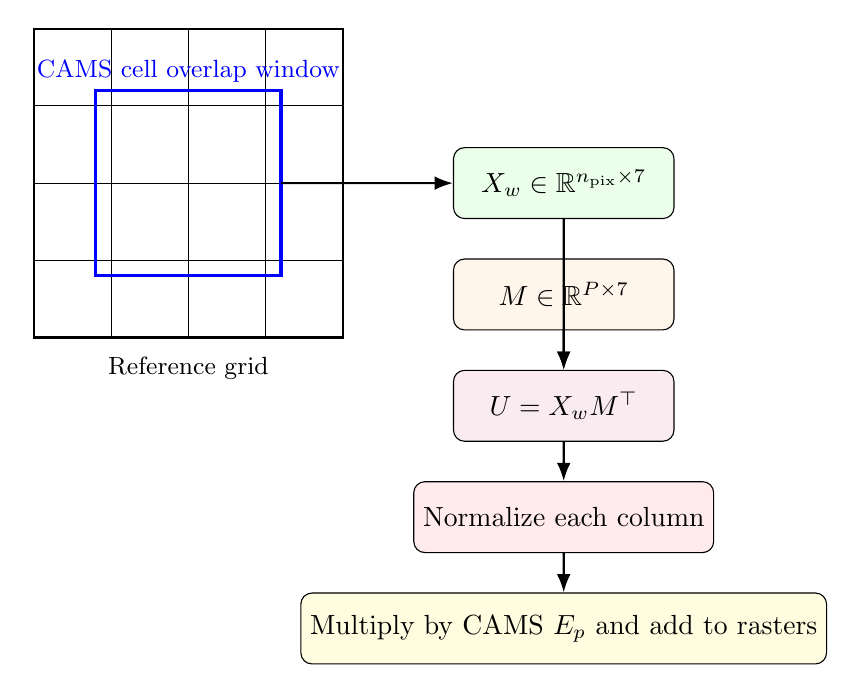
\begin{tikzpicture}[scale=0.98,
  cell/.style={draw, minimum width=0.95cm, minimum height=0.95cm, inner sep=0pt},
  lbl/.style={font=\small},
  arr/.style={-Latex, thick}
]

\draw[thick] (0,0) rectangle (4,4);
\foreach \x in {1,2,3} \draw (\x,0)--(\x,4);
\foreach \y in {1,2,3} \draw (0,\y)--(4,\y);
\draw[very thick, blue] (0.8,0.8) rectangle (3.2,3.2);
\node[lbl, blue] at (2,3.45) {CAMS cell overlap window};
\node[lbl] at (2,-0.4) {Reference grid};
\coordinate (gridright) at (4,2);

\node[draw, rounded corners, fill=green!8, minimum width=2.8cm, minimum height=0.9cm, right=1.4cm of gridright] (xw) {$X_w \in \R^{n_{\mathrm{pix}} \times 7}$};
\node[draw, rounded corners, fill=orange!8, minimum width=2.8cm, minimum height=0.9cm, below=0.5cm of xw] (m) {$M \in \R^{P \times 7}$};
\node[draw, rounded corners, fill=purple!8, minimum width=2.8cm, minimum height=0.9cm, below=0.5cm of m] (u) {$U = X_w M^\top$};
\node[draw, rounded corners, fill=red!8, minimum width=2.8cm, minimum height=0.9cm, below=0.5cm of u] (w) {Normalize each column};
\node[draw, rounded corners, fill=yellow!12, minimum width=3.4cm, minimum height=0.9cm, below=0.5cm of w] (a) {Multiply by CAMS $E_p$ and add to rasters};

\draw[arr] (3.2,2) -- (xw.west);
\draw[arr] (xw) -- (u);
\draw[arr] (m) -- (u);
\draw[arr] (u) -- (w);
\draw[arr] (w) -- (a);

\end{tikzpicture}
\caption{For each CAMS source cell, the windowed proxy tensor $X_w$ is combined with the country matrix $M$,
then normalized by pollutant and accumulated on the output grid.}
\end{figure}

\section{Toy numerical example}

Suppose one CAMS cell overlaps 3 reference pixels, and we inspect one pollutant $p$.
Assume the local matrix product gives:
\[
U_{\cdot,p} = \begin{bmatrix} 2.0 \\ 3.0 \\ 5.0 \end{bmatrix}.
\]

Then the sum is $S_p = 10$, so the local shares are
\[
\widetilde{w}_{\cdot,p} =
\begin{bmatrix}
0.2 \\ 0.3 \\ 0.5
\end{bmatrix}.
\]

If the CAMS emission of pollutant $p$ for that cell is
\[
E_p = 40\ \mathrm{kg/yr},
\]
the emission contributions added to the three pixels are
\[
\Delta A_{\cdot,p} =
\begin{bmatrix}
8 \\ 12 \\ 20
\end{bmatrix}\ \mathrm{kg/yr}.
\]

At the same time, the weight raster receives
\[
\Delta W_{\cdot,p} =
\begin{bmatrix}
0.2 \\ 0.3 \\ 0.5
\end{bmatrix}.
\]

If a later CAMS cell also overlaps these same pixels, its local normalized shares are
added on top. This is why the final weight raster is an accumulated influence field,
not a one-shot normalized partition.

\section{Fallback logic}

The main fallback paths implemented in code are:

\begin{itemize}[leftmargin=1.4em]
  \item If Eurostat is disabled, all end-use multipliers are 1.
  \item If the Eurostat geo label cannot be resolved, the same uniform fallback is used.
  \item If commercial alpha from \texttt{nrg\_bal\_s} is missing, the code uses $\alpha=0$.
  \item If residential Eurostat TJ values are missing or non-positive, the code uses a flat residential split.
  \item If a GAINS file is missing for a country, that country's $M$ is the zero matrix.
  \item If a pollutant column of $U$ has non-positive or non-finite sum, the allocator uses a uniform pixel split within the cell window.
  \item If a CAMS emission value is non-finite, it is replaced by zero before accumulation.
\end{itemize}

\section{What the final per-pollutant weights mean}

The phrase ``final per-pollutant weights'' can be understood at two levels:

\subsection{Local meaning inside one CAMS cell}

For one cell $m$ and pollutant $p$, the code constructs a probability-like vector
\[
\widetilde{w}^{(m)}_{\cdot,p}
\]
over that cell's overlapping reference pixels. This vector always sums to 1
(unless the cell is skipped because it does not overlap the domain).

\subsection{Meaning of the saved weight GeoTIFF band}

The output raster band for pollutant $p$ is the sum of those local vectors over all
processed cells:
\[
W_{p,q} = \sum_{m \in \mathcal{C}(q)} \widetilde{w}^{(m)}_{j(q,m),p}.
\]

So a large value of $W_{p,q}$ means:

\begin{quote}
Pixel $q$ repeatedly receives a large fraction of the within-cell allocation for pollutant $p$
across many CAMS source cells.
\end{quote}

This is exactly what the code writes to the multiband weight raster.

\section{Summary in plain language}

The code first builds a map of where each combustion class is likely to occur
($X$), then builds a table of how strongly each class contributes to each pollutant
($M$). For each CAMS source cell, it combines those two pieces into a pixel-level
score $U$, normalizes by pollutant so the cell's mass is split across its overlap
window, multiplies by the CAMS emission itself, and adds the result to the output
rasters. The final pollutant-specific weight raster is therefore the accumulated sum
of all these local within-cell shares.

\end{document}
